\documentclass{article}
\usepackage[T2A]{fontenc}
\usepackage[utf8]{inputenc}
\usepackage{graphicx}
\usepackage[export]{adjustbox}
\usepackage{geometry}
\usepackage{float}
\usepackage{indentfirst}
\usepackage{listings}


% \graphicspath{ {./img_fixed/} }

\geometry{verbose,a4paper,tmargin=2cm,bmargin=2cm,lmargin=2.5cm,rmargin=1.5cm}

% \overfullrule=2cm
\newcommand{\paragraphline}[1]{\paragraph{#1}\mbox{}\\}

\begin{document}

\begin{center}
\hfill \break
\large{МИНОБРНАУКИ РОССИИ}\\
\footnotesize{ФЕДЕРАЛЬНОЕ ГОСУДАРСТВЕННОЕ БЮДЖЕТНОЕ ОБРАЗОВАТЕЛЬНОЕ УЧРЕЖДЕНИЕ}\\ 
\footnotesize{ВЫСШЕГО ПРОФЕССИОНАЛЬНОГО ОБРАЗОВАНИЯ}\\
\small{\textbf{«ВОРОНЕЖСКИЙ ГОСУДАРСТВЕННЫЙ УНИВЕРСИТЕТ»}}\\
\hfill \break
\normalsize{Факультет компьютерных наук}\\
    \hfill \break
\normalsize{Кафедра программирования и информационных технологий}\\
\hfill\break
\hfill \break
\hfill \break
\hfill \break
\large{Отчет по предмету Архитектура информационных систем
\\1 лабораторная работа
\\Приложение для автоматизированного проведения тестирования}\\
\end{center}

\hfill \break
\hfill \break
\hfill \break
\hfill \break
\hfill \break

\begin{flushright} Вычиков Д.Д \end{flushright}
\vspace*{\fill}
\begin{center} Воронеж 2019 \end{center}
\thispagestyle{empty}
\newpage

\section{Диаграмма сущность-связь}
\begin{figure}[H]
    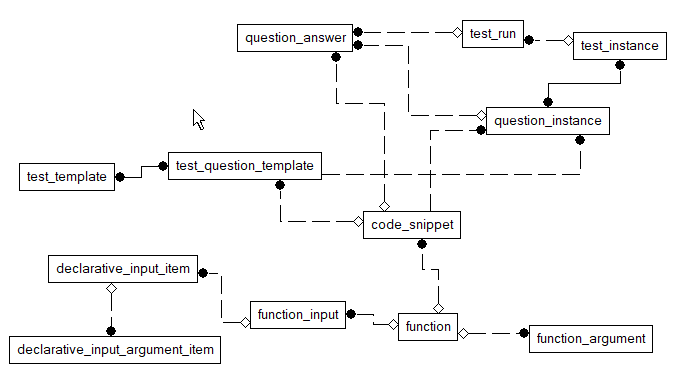
\includegraphics[width=\textwidth, center]{conceptual.png}
    \caption{Диаграмма сущность-связь}
\end{figure}
На диаграмма отображены следующие сущности:
\begin{enumerate}
    \item test\_template - Шаблон теста
    \item test\_question\_template - Шаблон вопроса
    \item code\_snippet - Объект для представления кода процедуры
    \item test\_instance - Тестовое событие
    \item question\_instance - Вопрос, принадлежащий тестовому
    событию
    \item test\_run - Прохожение тестирования
    \item question\_answer - Ответ на вопрос теста
    \item function - Процедура
    \item function\_argument - Аргумент процедуры
    \item function\_input - Набор тестовых параметров процедуры
    \item declarative\_input\_item
    \item declarative\_input\_argument\_item
\end{enumerate}

\section{Сгенерированный код}
\begin{lstlisting}
    
CREATE TABLE code_snippet
(
	id  integer NOT NULL,
	language  INTEGER NULL,
	code  text(65535) NULL,
	function_id  integer NULL
)
;



ALTER TABLE code_snippet
	ADD  PRIMARY KEY (id)
;



CREATE TABLE declarative_input_argument_item
(
	id  integer NOT NULL,
	argument_index  integer NULL,
	input_type  VARCHAR(20) NULL,
	input_value  text(65535) NULL,
	declarative_input_item_id  integer NULL
)
;



ALTER TABLE declarative_input_argument_item
	ADD  PRIMARY KEY (id)
;



CREATE TABLE declarative_input_item
(
	id  integer NOT NULL,
	output_value  text(65535) NULL,
	declarative_function_input_id  integer NULL
)
;



ALTER TABLE declarative_input_item
	ADD  PRIMARY KEY (id)
;



CREATE TABLE function
(
	id  integer NOT NULL,
	name  varchar(100) NULL,
	return_type  char(13) NULL
)
;



ALTER TABLE function
	ADD  PRIMARY KEY (id)
;



CREATE TABLE function_argument
(
	id  integer NOT NULL,
	type  char(13) NULL,
	name  varchar(100) NULL,
	function_id  integer NULL
)
;



ALTER TABLE function_argument
	ADD  PRIMARY KEY (id)
;



CREATE TABLE function_input
(
	id  integer NOT NULL,
	type  varchar(50) NULL,
	target_function_id  integer NULL
)
;



ALTER TABLE function_input
	ADD  PRIMARY KEY (id)
;



CREATE TABLE question_answer
(
	id  integer NOT NULL,
	is_validated  tinyint NULL,
	validation_passed  tinyint NULL,
	test_run_id  integer NULL,
	question_instance_id  integer NULL,
	code_snippet_id  integer NULL
)
;



ALTER TABLE question_answer
	ADD  PRIMARY KEY (id)
;



CREATE TABLE question_instance
(
	id  integer NOT NULL,
	name  varchar(100) NULL,
	time_limit  integer NULL,
	description  text(65535) NULL,
	parent_version  bigint NOT NULL,
	solution_code_snippet_id  integer NOT NULL,
	parent_id  integer NOT NULL
)
;



ALTER TABLE question_instance
	ADD  PRIMARY KEY (id)
;



CREATE TABLE test_instance
(
	id  integer NOT NULL,
	name  varchar(100) NULL,
	created_at  datetime NULL,
	available_after  datetime NULL,
	disabled_after  datetime NULL,
	time_limit  integer NULL,
	is_active  tinyint NULL
)
;



ALTER TABLE test_instance
	ADD  PRIMARY KEY (id)
;



CREATE TABLE test_instance_to_question_instance_association
(
	test_instance_id  integer NULL,
	question_instance_id  integer NULL
)
;



CREATE TABLE test_question_template
(
	id  integer NOT NULL,
	name  varchar(100) NULL,
	description  text(65535) NULL,
	time_limit  integer NULL,
	version  bigint NULL,
	is_deleted  tinyint NULL,
	solution_code_snippet_id  integer NULL
)
;



ALTER TABLE test_question_template
	ADD  PRIMARY KEY (id)
;



CREATE TABLE test_run
(
	id  integer NOT NULL,
	started_at  datetime NULL,
	finished_at  datetime NULL,
	ends_at  datetime NULL,
	test_instance_id  integer NULL
)
;



ALTER TABLE test_run
	ADD  PRIMARY KEY (id)
;



CREATE TABLE test_template
(
	id  integer NOT NULL,
	name  varchar(100) NULL,
	time_limit  integer NULL,
	is_deleted  tinyint NULL
)
;



ALTER TABLE test_template
	ADD  PRIMARY KEY (id)
;



CREATE TABLE test_template_test_question_template_association
(
	test_template_id  integer NULL,
	test_question_template_id  integer NULL
)
;



ALTER TABLE code_snippet
	ADD FOREIGN KEY code_snippet_ibfk_1 (function_id) REFERENCES function(id)
;



ALTER TABLE declarative_input_argument_item
	ADD FOREIGN KEY declarative_input_argument_item_ibfk_1 (declarative_input_item_id) REFERENCES declarative_input_item(id)
;



ALTER TABLE declarative_input_item
	ADD FOREIGN KEY declarative_input_item_ibfk_1 (declarative_function_input_id) REFERENCES function_input(id)
;



ALTER TABLE function_argument
	ADD FOREIGN KEY function_argument_ibfk_1 (function_id) REFERENCES function(id)
;



ALTER TABLE function_input
	ADD FOREIGN KEY function_input_ibfk_1 (target_function_id) REFERENCES function(id)
;



ALTER TABLE question_answer
	ADD FOREIGN KEY question_answer_ibfk_3 (code_snippet_id) REFERENCES code_snippet(id)
;


ALTER TABLE question_answer
	ADD FOREIGN KEY question_answer_ibfk_2 (question_instance_id) REFERENCES question_instance(id)
;


ALTER TABLE question_answer
	ADD FOREIGN KEY question_answer_ibfk_1 (test_run_id) REFERENCES test_run(id)
;



ALTER TABLE question_instance
	ADD FOREIGN KEY question_instance_ibfk_2 (parent_id) REFERENCES test_question_template(id)
;


ALTER TABLE question_instance
	ADD FOREIGN KEY question_instance_ibfk_1 (solution_code_snippet_id) REFERENCES code_snippet(id)
;



ALTER TABLE test_instance_to_question_instance_association
	ADD FOREIGN KEY test_instance_to_question_instance_association_ibfk_2 (question_instance_id) REFERENCES question_instance(id)
;


ALTER TABLE test_instance_to_question_instance_association
	ADD FOREIGN KEY test_instance_to_question_instance_association_ibfk_1 (test_instance_id) REFERENCES test_instance(id)
;



ALTER TABLE test_question_template
	ADD FOREIGN KEY test_question_template_ibfk_1 (solution_code_snippet_id) REFERENCES code_snippet(id)
;



ALTER TABLE test_run
	ADD FOREIGN KEY test_run_ibfk_1 (test_instance_id) REFERENCES test_instance(id)
;



ALTER TABLE test_template_test_question_template_association
	ADD FOREIGN KEY test_template_test_question_template_association_ibfk_2 (test_question_template_id) REFERENCES test_question_template(id)
;


ALTER TABLE test_template_test_question_template_association
	ADD FOREIGN KEY test_template_test_question_template_association_ibfk_1 (test_template_id) REFERENCES test_template(id)
;



\end{lstlisting}
\end{document}
